\pdfoutput=1
%% Author: PGL  Porta Mana, ALS Filipowicz
%% Created: 2018-04-08T16:54:19+0200
%% Last-Updated: 2018-04-17T22:37:59+0200
%%%%%%%%%%%%%%%%%%%%%%%%%%%%%%%%%%%%%%%%%%%%%%%%%%%%%%%%%%%%%%%%%%%%%%
% Report-no: ***
\newif\ifarxiv
\arxivfalse
\ifarxiv\pdfmapfile{+classico.map}\fi
\newif\ifafour
\afourfalse % true = A4, false = A5
\newif\iftypodisclaim % typographical disclaim on the side
\typodisclaimtrue
\newif\ifpublic
\publictrue % true = for publication, false = personal notes
\newcommand*{\memfontfamily}{zplx}
\newcommand*{\memfontpack}{newpxtext}
\documentclass[\ifafour a4paper,12pt,\else a5paper,10pt,\fi%extrafontsizes,%
onecolumn,oneside,article,%french,italian,german,swedish,latin,
british%
]{memoir}
\newcommand*{\oggi}{\today}
\newcommand*{\firstdraft}{14 April 2018}
\newcommand*{\firstpublished}{\oggi}
\newcommand*{\propertitle}{Bayesian Plinko\\{\large Study notes}}
\newcommand*{\pdftitle}{Bayesian Plinko}
\newcommand*{\headtitle}{Bayesian Plinko}
\newcommand*{\pdfauthor}{A. L. S. Filipowicz, P.G.L.  Porta Mana}
\newcommand*{\headauthor}{\ifpublic Filipowicz \amp\ Porta Mana%
\else\autanet\ Luca\fi}
\newcommand*{\reporthead}{}
%%%%%%%%%%%%%%%%%%%%%%%%%%%%%%%%%%%%%%%%%%%%%%%%%%%%%%%%%%%%%%%%%%%%%%%%%%%%
%%%%%%%%%%%%%%%%%%%%%%%%%%%%%%%%%%%%%%%%%%%%%%%%%%%%%%%%%%%%%%%%%%%%%%%%%%%%
%\usepackage{pifont}
%\usepackage{fontawesome}
\usepackage[T1]{fontenc} 
\input{glyphtounicode} \pdfgentounicode=1
\usepackage[utf8]{inputenx}
%\usepackage{newunicodechar}
% \newunicodechar{Ĕ}{\u{E}}
% \newunicodechar{ĕ}{\u{e}}
% \newunicodechar{Ĭ}{\u{I}}
% \newunicodechar{ĭ}{\u{\i}}
% \newunicodechar{Ŏ}{\u{O}}
% \newunicodechar{ŏ}{\u{o}}
% \newunicodechar{Ŭ}{\u{U}}
% \newunicodechar{ŭ}{\u{u}}
% \newunicodechar{Ā}{\=A}
% \newunicodechar{ā}{\=a}
% \newunicodechar{Ē}{\=E}
% \newunicodechar{ē}{\=e}
% \newunicodechar{Ī}{\=I}
% \newunicodechar{ī}{\={\i}}
% \newunicodechar{Ō}{\=O}
% \newunicodechar{ō}{\=o}
% \newunicodechar{Ū}{\=U}
% \newunicodechar{ū}{\=u}
% \newunicodechar{Ȳ}{\=Y}
% \newunicodechar{ȳ}{\=y}

\newcommand*{\bmmax}{0} % reduce number of bold fonts, before bm
\newcommand*{\hmmax}{0} % reduce number of heavy fonts, before bm
\usepackage{textcomp}
\usepackage[normalem]{ulem}
% \makeatletter
% \def\ssout{\bgroup \ULdepth=-.35ex%\UL@setULdepth
%  \markoverwith{\lower\ULdepth\hbox
%    {\kern-.03em\vbox{\hrule width.2em\kern1.2\p@\hrule}\kern-.03em}}%
%  \ULon}
% \makeatother
\usepackage{amsmath}
\usepackage{mathtools}
\usepackage{empheq}% automatically calls amsmath and mathtools
\newcommand*{\widefbox}[1]{\fbox{\hspace{1em}#1\hspace{1em}}}
\setlength{\multlinegap}{0pt}
%\usepackage{fancybox}
\usepackage{framed}
% \usepackage[misc]{ifsym} % for dice
% \newcommand*{\diceone}{{\scriptsize\Cube{1}}}
\usepackage{amssymb}
\usepackage{amsxtra}

\usepackage[main=british,french,italian,german,swedish,latin,esperanto]{babel}\selectlanguage{british}
\newcommand*{\langfrench}{\foreignlanguage{french}}
\newcommand*{\langgerman}{\foreignlanguage{german}}
\newcommand*{\langitalian}{\foreignlanguage{italian}}
\newcommand*{\langswedish}{\foreignlanguage{swedish}}
\newcommand*{\langlatin}{\foreignlanguage{latin}}
\newcommand*{\langnohyph}{\foreignlanguage{nohyphenation}}

\usepackage[autostyle=false,autopunct=false,english=british]{csquotes}
\setquotestyle{british}

\usepackage{amsthm}
\newcommand*{\QED}{\textsc{q.e.d.}}
\renewcommand*{\qedsymbol}{\QED}
\theoremstyle{remark}
\newtheorem{note}{Note}
\newtheorem*{remark}{Note}
\newtheoremstyle{innote}{\parsep}{\parsep}{\footnotesize}{}{}{}{0pt}{}
\theoremstyle{innote}
\newtheorem*{innote}{}


\usepackage[shortlabels,inline]{enumitem}
\SetEnumitemKey{para}{itemindent=\parindent,leftmargin=0pt,listparindent=\parindent,parsep=0pt,itemsep=\topsep}
% \begin{asparaenum} = \begin{enumerate}[para]
% \begin{inparaenum} = \begin{enumerate*}
\setlist[enumerate,2]{label=\alph*.}
\setlist[enumerate]{leftmargin=\parindent}
\setlist[itemize]{leftmargin=\parindent}
\setlist[description]{leftmargin=\parindent}

\usepackage[babel,theoremfont]{newpxtext}
\usepackage[bigdelims,nosymbolsc%,smallerops % probably arXiv doesn't have it
]{newpxmath}
\useosf\linespread{1.083}
%% smaller operators for old version of newpxmath
\makeatletter
\def\re@DeclareMathSymbol#1#2#3#4{%
    \let#1=\undefined
    \DeclareMathSymbol{#1}{#2}{#3}{#4}}
%\re@DeclareMathSymbol{\bigsqcupop}{\mathop}{largesymbols}{"46}
%\re@DeclareMathSymbol{\bigodotop}{\mathop}{largesymbols}{"4A}
\re@DeclareMathSymbol{\bigoplusop}{\mathop}{largesymbols}{"4C}
\re@DeclareMathSymbol{\bigotimesop}{\mathop}{largesymbols}{"4E}
\re@DeclareMathSymbol{\sumop}{\mathop}{largesymbols}{"50}
\re@DeclareMathSymbol{\prodop}{\mathop}{largesymbols}{"51}
\re@DeclareMathSymbol{\bigcupop}{\mathop}{largesymbols}{"53}
\re@DeclareMathSymbol{\bigcapop}{\mathop}{largesymbols}{"54}
%\re@DeclareMathSymbol{\biguplusop}{\mathop}{largesymbols}{"55}
\re@DeclareMathSymbol{\bigwedgeop}{\mathop}{largesymbols}{"56}
\re@DeclareMathSymbol{\bigveeop}{\mathop}{largesymbols}{"57}
%\re@DeclareMathSymbol{\bigcupdotop}{\mathop}{largesymbols}{"DF}
%\re@DeclareMathSymbol{\bigcapplusop}{\mathop}{largesymbolsPXA}{"00}
%\re@DeclareMathSymbol{\bigsqcupplusop}{\mathop}{largesymbolsPXA}{"02}
%\re@DeclareMathSymbol{\bigsqcapplusop}{\mathop}{largesymbolsPXA}{"04}
%\re@DeclareMathSymbol{\bigsqcapop}{\mathop}{largesymbolsPXA}{"06}
\re@DeclareMathSymbol{\bigtimesop}{\mathop}{largesymbolsPXA}{"10}
%\re@DeclareMathSymbol{\coprodop}{\mathop}{largesymbols}{"60}
%\re@DeclareMathSymbol{\varprod}{\mathop}{largesymbolsPXA}{16}
\makeatother


%% With euler font cursive for Greek letters - the [1] means 100% scaling
\DeclareFontFamily{U}{egreek}{\skewchar\font'177}%
\DeclareFontShape{U}{egreek}{m}{n}{<-6>s*[1]eurm5 <6-8>s*[1]eurm7 <8->s*[1]eurm10}{}%
\DeclareFontShape{U}{egreek}{m}{it}{<->s*[1]eurmo10}{}%
\DeclareFontShape{U}{egreek}{b}{n}{<-6>s*[1]eurb5 <6-8>s*[1]eurb7 <8->s*[1]eurb10}{}%
\DeclareFontShape{U}{egreek}{b}{it}{<->s*[1]eurbo10}{}%
\DeclareSymbolFont{egreeki}{U}{egreek}{m}{it}%
\SetSymbolFont{egreeki}{bold}{U}{egreek}{b}{it}% from the amsfonts package
\DeclareSymbolFont{egreekr}{U}{egreek}{m}{n}%
\SetSymbolFont{egreekr}{bold}{U}{egreek}{b}{n}% from the amsfonts package
% Take also \sum, \prod, \coprod symbols from Euler fonts
\DeclareFontFamily{U}{egreekx}{\skewchar\font'177}
\DeclareFontShape{U}{egreekx}{m}{n}{%
       <-7.5>s*[0.9]euex7%
    <7.5-8.5>s*[0.9]euex8%
    <8.5-9.5>s*[0.9]euex9%
    <9.5->s*[0.9]euex10%
}{}
\DeclareSymbolFont{egreekx}{U}{egreekx}{m}{n}
\DeclareMathSymbol{\sumop}{\mathop}{egreekx}{"50}
\DeclareMathSymbol{\prodop}{\mathop}{egreekx}{"51}
\DeclareMathSymbol{\coprodop}{\mathop}{egreekx}{"60}
\makeatletter
\def\sum{\DOTSI\sumop\slimits@}
\def\prod{\DOTSI\prodop\slimits@}
\def\coprod{\DOTSI\coprodop\slimits@}
\makeatother
\ifarxiv\else\let\varpartial\undefined
\let\partialup\undefined
\let\alpha\undefined
\let\beta\undefined
\let\gamma\undefined
\let\delta\undefined
\let\epsilon\undefined
\let\zeta\undefined
\let\eta\undefined
\let\theta\undefined
\let\iota\undefined
\let\kappa\undefined
\let\lambda\undefined
\let\mu\undefined
\let\nu\undefined
\let\xi\undefined
\let\omicron\undefined
\let\pi\undefined
\let\rho\undefined
\let\sigma\undefined
\let\tau\undefined
\let\upsilon\undefined
\let\phi\undefined
\let\chi\undefined
\let\psi\undefined
\let\omega\undefined
\let\varepsilon\undefined
\let\vartheta\undefined
\let\varpi\undefined
\let\varrho\undefined 
\let\varsigma\undefined
\let\varkappa\undefined
\let\varphi\undefined
%
\let\varAlpha\undefined
\let\varBeta\undefined
\let\varGamma\undefined
\let\varDelta\undefined
\let\varEpsilon\undefined
\let\varZeta\undefined
\let\varEta\undefined
\let\varTheta\undefined
\let\varIota\undefined
\let\varKappa\undefined
\let\varLambda\undefined
\let\varMu\undefined
\let\varNu\undefined
\let\varXi\undefined
\let\varOmicron\undefined
\let\varPi\undefined
\let\varRho\undefined
\let\varSigma\undefined
\let\varTau\undefined
\let\varUpsilon\undefined
\let\varPhi\undefined
\let\varChi\undefined
\let\varPsi\undefined
\let\varOmega\undefined
%
\let\Alpha\undefined
\let\Beta\undefined
\let\Gamma\undefined
\let\Delta\undefined
\let\Epsilon\undefined
\let\Zeta\undefined
\let\Eta\undefined
\let\Theta\undefined
\let\Iota\undefined
\let\Kappa\undefined
\let\Lambda\undefined
\let\Mu\undefined
\let\Nu\undefined
\let\Xi\undefined
\let\Omicron\undefined
\let\Pi\undefined
\let\Rho\undefined
\let\Sigma\undefined
\let\Tau\undefined
\let\Upsilon\undefined
\let\Phi\undefined
\let\Chi\undefined
\let\Psi\undefined
\let\Omega\undefined
%
\let\alphaup\undefined
\let\betaup\undefined
\let\gammaup\undefined
\let\deltaup\undefined
\let\epsilonup\undefined
\let\zetaup\undefined
\let\etaup\undefined
\let\thetaup\undefined
\let\iotaup\undefined
\let\kappaup\undefined
\let\lambdaup\undefined
\let\muup\undefined
\let\nuup\undefined
\let\xiup\undefined
\let\omicronup\undefined
\let\piup\undefined
\let\rhoup\undefined
\let\sigmaup\undefined
\let\tauup\undefined
\let\upsilonup\undefined
\let\phiup\undefined
\let\chiup\undefined
\let\psiup\undefined
\let\omegaup\undefined
\let\varepsilonup\undefined
\let\varthetaup\undefined
\let\varpiup\undefined
\let\varrhoup\undefined
\let\varsigmaup\undefined
\let\varkappaup\undefined
\let\varphiup\undefined
\fi% make sure no CMF greek letters sneak in
% Greek letters not usually given in LaTeX. Comment the unneeded ones
% \DeclareMathSymbol{\varpartial}{\mathalpha}{egreeki}{"40}
 \DeclareMathSymbol{\partialup}{\mathalpha}{egreekr}{"40}
% \DeclareMathSymbol{\alpha}{\mathalpha}{egreeki}{"0B}
% \DeclareMathSymbol{\beta}{\mathalpha}{egreeki}{"0C}
% \DeclareMathSymbol{\gamma}{\mathalpha}{egreeki}{"0D}
% \DeclareMathSymbol{\delta}{\mathalpha}{egreeki}{"0E}
 \DeclareMathSymbol{\epsilon}{\mathalpha}{egreeki}{"0F}
% \DeclareMathSymbol{\zeta}{\mathalpha}{egreeki}{"10}
% \DeclareMathSymbol{\eta}{\mathalpha}{egreeki}{"11}
% \DeclareMathSymbol{\theta}{\mathalpha}{egreeki}{"12}
% \DeclareMathSymbol{\iota}{\mathalpha}{egreeki}{"13}
 \DeclareMathSymbol{\kappa}{\mathalpha}{egreeki}{"14}
 \DeclareMathSymbol{\lambda}{\mathalpha}{egreeki}{"15}
% \DeclareMathSymbol{\mu}{\mathalpha}{egreeki}{"16}
 \DeclareMathSymbol{\nu}{\mathalpha}{egreeki}{"17}
% \DeclareMathSymbol{\xi}{\mathalpha}{egreeki}{"18}
% \DeclareMathSymbol{\omicron}{\mathalpha}{egreeki}{"6F}
% \DeclareMathSymbol{\pi}{\mathalpha}{egreeki}{"19}
% \DeclareMathSymbol{\rho}{\mathalpha}{egreeki}{"1A}
% \DeclareMathSymbol{\sigma}{\mathalpha}{egreeki}{"1B}
% \DeclareMathSymbol{\tau}{\mathalpha}{egreeki}{"1C}
% \DeclareMathSymbol{\upsilon}{\mathalpha}{egreeki}{"1D}
% \DeclareMathSymbol{\phi}{\mathalpha}{egreeki}{"1E}
% \DeclareMathSymbol{\chi}{\mathalpha}{egreeki}{"1F}
% \DeclareMathSymbol{\psi}{\mathalpha}{egreeki}{"20}
% \DeclareMathSymbol{\omega}{\mathalpha}{egreeki}{"21}
% \DeclareMathSymbol{\varepsilon}{\mathalpha}{egreeki}{"22}
% \DeclareMathSymbol{\vartheta}{\mathalpha}{egreeki}{"23}
% \DeclareMathSymbol{\varpi}{\mathalpha}{egreeki}{"24}
% \let\varrho\rho 
% \let\varsigma\sigma
 \let\varkappa\kappa
% \DeclareMathSymbol{\varphi}{\mathalpha}{egreeki}{"27}
% %
% \DeclareMathSymbol{\varAlpha}{\mathalpha}{egreeki}{"41}
% \DeclareMathSymbol{\varBeta}{\mathalpha}{egreeki}{"42}
% \DeclareMathSymbol{\varGamma}{\mathalpha}{egreeki}{"00}
 \DeclareMathSymbol{\varDelta}{\mathalpha}{egreeki}{"01}
 \DeclareMathSymbol{\varEpsilon}{\mathalpha}{egreeki}{"45}
% \DeclareMathSymbol{\varZeta}{\mathalpha}{egreeki}{"5A}
% \DeclareMathSymbol{\varEta}{\mathalpha}{egreeki}{"48}
% \DeclareMathSymbol{\varTheta}{\mathalpha}{egreeki}{"02}
 \DeclareMathSymbol{\varIota}{\mathalpha}{egreeki}{"49}
% \DeclareMathSymbol{\varKappa}{\mathalpha}{egreeki}{"4B}
 \DeclareMathSymbol{\varLambda}{\mathalpha}{egreeki}{"03}
% \DeclareMathSymbol{\varMu}{\mathalpha}{egreeki}{"4D}
% \DeclareMathSymbol{\varNu}{\mathalpha}{egreeki}{"4E}
% \DeclareMathSymbol{\varXi}{\mathalpha}{egreeki}{"04}
% \DeclareMathSymbol{\varOmicron}{\mathalpha}{egreeki}{"4F}
% \DeclareMathSymbol{\varPi}{\mathalpha}{egreeki}{"05}
% \DeclareMathSymbol{\varRho}{\mathalpha}{egreeki}{"50}
% \DeclareMathSymbol{\varSigma}{\mathalpha}{egreeki}{"06}
% \DeclareMathSymbol{\varTau}{\mathalpha}{egreeki}{"54}
% \DeclareMathSymbol{\varUpsilon}{\mathalpha}{egreeki}{"07}
% \DeclareMathSymbol{\varPhi}{\mathalpha}{egreeki}{"08}
% \DeclareMathSymbol{\varChi}{\mathalpha}{egreeki}{"58}
% \DeclareMathSymbol{\varPsi}{\mathalpha}{egreeki}{"09}
% \DeclareMathSymbol{\varOmega}{\mathalpha}{egreeki}{"0A} 
% %
% \DeclareMathSymbol{\Alpha}{\mathalpha}{egreekr}{"41}
% \DeclareMathSymbol{\Beta}{\mathalpha}{egreekr}{"42}
 \DeclareMathSymbol{\Gamma}{\mathalpha}{egreekr}{"00}
% \DeclareMathSymbol{\Delta}{\mathalpha}{egreekr}{"01}
% \DeclareMathSymbol{\Epsilon}{\mathalpha}{egreekr}{"45}
% \DeclareMathSymbol{\Zeta}{\mathalpha}{egreekr}{"5A}
% \DeclareMathSymbol{\Eta}{\mathalpha}{egreekr}{"48}
% \DeclareMathSymbol{\Theta}{\mathalpha}{egreekr}{"02}
% \DeclareMathSymbol{\Iota}{\mathalpha}{egreekr}{"49}
% \DeclareMathSymbol{\Kappa}{\mathalpha}{egreekr}{"4B}
% \DeclareMathSymbol{\Lambda}{\mathalpha}{egreekr}{"03}
% \DeclareMathSymbol{\Mu}{\mathalpha}{egreekr}{"4D}
% \DeclareMathSymbol{\Nu}{\mathalpha}{egreekr}{"4E}
% \DeclareMathSymbol{\Xi}{\mathalpha}{egreekr}{"04}
% \DeclareMathSymbol{\Omicron}{\mathalpha}{egreekr}{"4F}
% \DeclareMathSymbol{\Pi}{\mathalpha}{egreekr}{"05}
% \DeclareMathSymbol{\Rho}{\mathalpha}{egreekr}{"50}
% \DeclareMathSymbol{\Sigma}{\mathalpha}{egreekr}{"06}
% \DeclareMathSymbol{\Tau}{\mathalpha}{egreekr}{"54}
% \DeclareMathSymbol{\Upsilon}{\mathalpha}{egreekr}{"07}
% \DeclareMathSymbol{\Phi}{\mathalpha}{egreekr}{"08}
% \DeclareMathSymbol{\Chi}{\mathalpha}{egreekr}{"58}
% \DeclareMathSymbol{\Psi}{\mathalpha}{egreekr}{"09}
% \DeclareMathSymbol{\Omega}{\mathalpha}{egreekr}{"0A}
% %
% \DeclareMathSymbol{\alphaup}{\mathalpha}{egreekr}{"0B}
% \DeclareMathSymbol{\betaup}{\mathalpha}{egreekr}{"0C}
% \DeclareMathSymbol{\gammaup}{\mathalpha}{egreekr}{"0D}
 \DeclareMathSymbol{\deltaup}{\mathalpha}{egreekr}{"0E}
% \DeclareMathSymbol{\epsilonup}{\mathalpha}{egreekr}{"0F}
% \DeclareMathSymbol{\zetaup}{\mathalpha}{egreekr}{"10}
% \DeclareMathSymbol{\etaup}{\mathalpha}{egreekr}{"11}
% \DeclareMathSymbol{\thetaup}{\mathalpha}{egreekr}{"12}
% \DeclareMathSymbol{\iotaup}{\mathalpha}{egreekr}{"13}
% \DeclareMathSymbol{\kappaup}{\mathalpha}{egreekr}{"14}
% \DeclareMathSymbol{\lambdaup}{\mathalpha}{egreekr}{"15}
% \DeclareMathSymbol{\muup}{\mathalpha}{egreekr}{"16}
% \DeclareMathSymbol{\nuup}{\mathalpha}{egreekr}{"17}
% \DeclareMathSymbol{\xiup}{\mathalpha}{egreekr}{"18}
% \DeclareMathSymbol{\omicronup}{\mathalpha}{egreekr}{"6F}
  \DeclareMathSymbol{\piup}{\mathalpha}{egreekr}{"19}
% \DeclareMathSymbol{\rhoup}{\mathalpha}{egreekr}{"1A}
% \DeclareMathSymbol{\sigmaup}{\mathalpha}{egreekr}{"1B}
% \DeclareMathSymbol{\tauup}{\mathalpha}{egreekr}{"1C}
% \DeclareMathSymbol{\upsilonup}{\mathalpha}{egreekr}{"1D}
% \DeclareMathSymbol{\phiup}{\mathalpha}{egreekr}{"1E}
% \DeclareMathSymbol{\chiup}{\mathalpha}{egreekr}{"1F}
% \DeclareMathSymbol{\psiup}{\mathalpha}{egreekr}{"20}
% \DeclareMathSymbol{\omegaup}{\mathalpha}{egreekr}{"21}
% \DeclareMathSymbol{\varepsilonup}{\mathalpha}{egreekr}{"22}
% \DeclareMathSymbol{\varthetaup}{\mathalpha}{egreekr}{"23}
% \DeclareMathSymbol{\varpiup}{\mathalpha}{egreekr}{"24}
% \let\varrhoup\rhoup 
% \let\varsigmaup\sigmaup
% \let\varkappaup\kappaup
% \DeclareMathSymbol{\varphiup}{\mathalpha}{egreekr}{"27}

% Optima as sans-serif font
%\usepackage%[scaled=0.9]%
%{classico}
\renewcommand\sfdefault{uop}
\DeclareMathAlphabet{\mathsf}  {T1}{\sfdefault}{m}{sl}
\SetMathAlphabet{\mathsf}{bold}{T1}{\sfdefault}{b}{sl}
\newcommand*{\mathte}[1]{\textbf{\textit{\textsf{#1}}}}
% Upright sans-serif math alphabet
% \DeclareMathAlphabet{\mathsu}  {T1}{\sfdefault}{m}{n}
% \SetMathAlphabet{\mathsu}{bold}{T1}{\sfdefault}{b}{n}

% DejaVu Mono as typewriter text
\usepackage[scaled=0.84]{DejaVuSansMono}


\usepackage{mathdots}

\usepackage[usenames]{xcolor}
% Tol (2012) colour-blind-, print-, screen-friendly colours; Munsell terminology
\definecolor{mybluishpurple}{RGB}{51,34,136}
\definecolor{myblue}{RGB}{136,204,238}
\definecolor{mybluishgreen}{RGB}{68,170,153}
\definecolor{mygreen}{RGB}{17,119,51}
\definecolor{mygreenishyellow}{RGB}{153,153,51}
\definecolor{myyellow}{RGB}{221,204,119}
\definecolor{myred}{RGB}{204,102,119}
\definecolor{mypurplishred}{RGB}{136,34,85}
\definecolor{myreddishpurple}{RGB}{170,68,153}
\definecolor{mygrey}{RGB}{221,221,221}
%\newcommand*\mycolourbox[1]{%
%\colorbox{mygrey}{\hspace{1em}#1\hspace{1em}}}
\colorlet{shadecolor}{mygrey}

\usepackage{bm}
\usepackage{microtype}

\usepackage[backend=biber,mcite,%subentry,
citestyle=authoryear-comp,bibstyle=pglpm-authoryear,autopunct=false,sorting=ny,sortcites=false,natbib=false,maxcitenames=1,maxbibnames=8,minbibnames=8,giveninits=true,uniquename=false,uniquelist=false,maxalphanames=1,block=space,hyperref=true,defernumbers=false,useprefix=true,sortupper=false,language=british,parentracker=false]{biblatex}
\DeclareSortingScheme{ny}{\sort{\field{sortname}\field{author}\field{editor}}\sort{\field{year}}}
\iffalse\makeatletter%%% replace parenthesis with brackets
\newrobustcmd*{\parentexttrack}[1]{%
  \begingroup
  \blx@blxinit
  \blx@setsfcodes
  \blx@bibopenparen#1\blx@bibcloseparen
  \endgroup}
\AtEveryCite{%
  \let\parentext=\parentexttrack%
  \let\bibopenparen=\bibopenbracket%
  \let\bibcloseparen=\bibclosebracket}
\makeatother\fi
\DefineBibliographyExtras{british}{\def\finalandcomma{\addcomma}}
\renewcommand*{\finalnamedelim}{\addcomma\space}
\setcounter{biburlnumpenalty}{1}
\setcounter{biburlucpenalty}{0}
\setcounter{biburllcpenalty}{1}
\DeclareDelimFormat{multicitedelim}{\addsemicolon\space}
\DeclareDelimFormat{compcitedelim}{\addsemicolon\space}
\DeclareDelimFormat{postnotedelim}{\space}
\ifarxiv\else\addbibresource{portamanabib.bib}\fi
\renewcommand{\bibfont}{\footnotesize}
\appto{\citesetup}{\footnotesize}% smaller font for citations
\defbibheading{bibliography}[\bibname]{\section*{#1}\addcontentsline{toc}{section}{#1}%\markboth{#1}{#1}
}
\newcommand*{\citep}{\parencites}
\newcommand*{\citey}{\parencites*}
%\renewcommand*{\cite}{\parencite}
\renewcommand*{\cites}{\parencites}
\providecommand{\href}[2]{#2}
\providecommand{\eprint}[2]{\texttt{\href{#1}{#2}}}
\newcommand*{\amp}{\&}
% \newcommand*{\citein}[2][]{\textnormal{\textcite[#1]{#2}}%\addtocategory{extras}{#2}
% }
\newcommand*{\citein}[2][]{\textnormal{\textcite[#1]{#2}}%\addtocategory{extras}{#2}
}
\newcommand*{\citebi}[2][]{\textcite[#1]{#2}%\addtocategory{extras}{#2}
}
\newcommand*{\subtitleproc}[1]{}
\newcommand*{\chapb}{ch.}

% \def\arxivp{}
% \def\mparcp{}
% \def\philscip{}
% \def\biorxivp{}
% \newcommand*{\arxivsi}{\texttt{arXiv} eprints available at \url{http://arxiv.org/}.\\}
% \newcommand*{\mparcsi}{\texttt{mp\_arc} eprints available at \url{http://www.ma.utexas.edu/mp_arc/}.\\}
% \newcommand*{\philscisi}{\texttt{philsci} eprints available at \url{http://philsci-archive.pitt.edu/}.\\}
% \newcommand*{\biorxivsi}{\texttt{bioRxiv} eprints available at \url{http://biorxiv.org/}.\\}
\newcommand*{\arxiveprint}[1]{%\global\def\arxivp{\arxivsi}%\citeauthor{0arxivcite}\addtocategory{ifarchcit}{0arxivcite}%eprint
\texttt{\urlalt{https://arxiv.org/abs/#1}{arXiv:\hspace{0pt}#1}}%
%\texttt{\href{http://arxiv.org/abs/#1}{\protect\url{arXiv:#1}}}%
%\renewcommand{\arxivnote}{\texttt{arXiv} eprints available at \url{http://arxiv.org/}.}
}
\newcommand*{\mparceprint}[1]{%\global\def\mparcp{\mparcsi}%\citeauthor{0mparccite}\addtocategory{ifarchcit}{0mparccite}%eprint
\texttt{\urlalt{http://www.ma.utexas.edu/mp_arc-bin/mpa?yn=#1}{mp\_arc:\hspace{0pt}#1}}%
%\texttt{\href{http://www.ma.utexas.edu/mp_arc-bin/mpa?yn=#1}{\protect\url{mp_arc:#1}}}%
%\providecommand{\mparcnote}{\texttt{mp_arc} eprints available at \url{http://www.ma.utexas.edu/mp_arc/}.}
}
\newcommand*{\philscieprint}[1]{%\global\def\philscip{\philscisi}%\citeauthor{0philscicite}\addtocategory{ifarchcit}{0philscicite}%eprint
\texttt{\urlalt{http://philsci-archive.pitt.edu/archive/#1}{PhilSci:\hspace{0pt}#1}}%
%\texttt{\href{http://philsci-archive.pitt.edu/archive/#1}{\protect\url{PhilSci:#1}}}%
%\providecommand{\mparcnote}{\texttt{philsci} eprints available at \url{http://philsci-archive.pitt.edu/}.}
}
\newcommand*{\biorxiveprint}[1]{%\global\def\biorxivp{\biorxivsi}%\citeauthor{0arxivcite}\addtocategory{ifarchcit}{0arxivcite}%eprint
\texttt{\urlalt{http://biorxiv.org/content/early/#1}{bioRxiv:\hspace{0pt}#1}}%
%\texttt{\href{http://arxiv.org/abs/#1}{\protect\url{arXiv:#1}}}%
%\renewcommand{\arxivnote}{\texttt{arXiv} eprints available at \url{http://arxiv.org/}.}
}
\newcommand*{\osfeprint}[1]{%
\texttt{\urlalt{https://doi.org/10.17605/osf.io/#1}{doi:10.17605/osf.io/#1}}%
}

\usepackage{graphicx}
\usepackage{wrapfig}

\PassOptionsToPackage{hyphens}{url}\usepackage[hypertexnames=false]{hyperref}
\usepackage[depth=4]{bookmark}
\hypersetup{colorlinks=true,bookmarksnumbered,pdfborder={0 0 0.25},citebordercolor={0.2 0.1333 0.5333},%bluish
citecolor=mybluishpurple,linkbordercolor={0.0667 0.4667 0.2},%greenish
linkcolor=mypurplishred,urlbordercolor={0.5333 0.1333 0.3333},%reddish
urlcolor=mygreen,breaklinks=true,pdftitle={\pdftitle},pdfauthor={\pdfauthor}}
% \usepackage[vertfit=local]{breakurl}% only for arXiv
\providecommand*{\urlalt}{\href}

%%% Layout. I do not know on which kind of paper the reader will print the
%%% paper on (A4? letter? one-sided? double-sided?). So I choose A5, which
%%% provides a good layout for reading on screen and save paper if printed
%%% two pages per sheet. Average length line is 66 characters and page
%%% numbers are centred.
\ifafour\setstocksize{297mm}{210mm}%{*}% A4
\else\setstocksize{210mm}{5.5in}%{*}% 210x139.7
\fi
\settrimmedsize{\stockheight}{\stockwidth}{*}
\setlxvchars[\normalfont] %313.3632pt for a 66-characters line
\setxlvchars[\normalfont]
\setlength{\trimtop}{0pt}
\setlength{\trimedge}{\stockwidth}
\addtolength{\trimedge}{-\paperwidth}
% The length of the normalsize alphabet is 133.05988pt - 10 pt = 26.1408pc
% The length of the normalsize alphabet is 159.6719pt - 12pt = 30.3586pc
% Bringhurst gives 32pc as boundary optimal with 69 ch per line
% The length of the normalsize alphabet is 191.60612pt - 14pt = 35.8634pc
\ifafour\settypeblocksize{*}{32pc}{1.618} % A4
%\setulmargins{*}{*}{1.667}%gives 5/3 margins % 2 or 1.667
\else\settypeblocksize{*}{26pc}{1.618}% nearer to a 66-line newpx and preserves GR
\fi
\setulmargins{*}{*}{1}%gives equal margins
\setlrmargins{*}{*}{*}
\setheadfoot{\onelineskip}{2.5\onelineskip}
\setheaderspaces{*}{2\onelineskip}{*}
\setmarginnotes{2ex}{10mm}{0pt}
\checkandfixthelayout[nearest]
\fixpdflayout
%%% End layout
%% this fixes missing white spaces
\pdfmapline{+dummy-space <dummy-space.pfb}\pdfinterwordspaceon%

%%% Sectioning
\newcommand*{\asudedication}[1]{%
{\par\centering\textit{#1}\par}}
\newenvironment{acknowledgements}{\section*{Thanks}\addcontentsline{toc}{section}{Thanks}}{\par}
\makeatletter\renewcommand{\appendix}{\par
  \bigskip{\centering
   \interlinepenalty \@M
   \normalfont
   \printchaptertitle{\sffamily\appendixpagename}\par}
  \setcounter{section}{0}%
  \gdef\@chapapp{\appendixname}%
  \gdef\thesection{\@Alph\c@section}%
  \anappendixtrue}\makeatother
\counterwithout{section}{chapter}
\setsecnumformat{\upshape\csname the#1\endcsname\quad}
\setsecheadstyle{\large\bfseries\sffamily%
\raggedright}
\setsubsecheadstyle{\bfseries\sffamily%
\raggedright}
%\setbeforesecskip{-1.5ex plus 1ex minus .2ex}% plus 1ex minus .2ex}
%\setaftersecskip{1.3ex plus .2ex }% plus 1ex minus .2ex}
%\setsubsubsecheadstyle{\bfseries\sffamily\slshape\raggedright}
%\setbeforesubsecskip{1.25ex plus 1ex minus .2ex }% plus 1ex minus .2ex}
%\setaftersubsecskip{-1em}%{-0.5ex plus .2ex}% plus 1ex minus .2ex}
\setsubsecindent{0pt}%0ex plus 1ex minus .2ex}
\setparaheadstyle{\bfseries\sffamily%
\raggedright}
\setcounter{secnumdepth}{2}
\setlength{\headwidth}{\textwidth}
\newcommand{\addchap}[1]{\chapter*[#1]{#1}\addcontentsline{toc}{chapter}{#1}}
\newcommand{\addsec}[1]{\section*{#1}\addcontentsline{toc}{section}{#1}}
\newcommand{\addsubsec}[1]{\subsection*{#1}\addcontentsline{toc}{subsection}{#1}}
\newcommand{\addpara}[1]{\paragraph*{#1.}\addcontentsline{toc}{subsubsection}{#1}}
\newcommand{\addparap}[1]{\paragraph*{#1}\addcontentsline{toc}{subsubsection}{#1}}

% Headers and footers
\copypagestyle{manaart}{plain}
\makeheadrule{manaart}{\headwidth}{0.5\normalrulethickness}
\makeoddhead{manaart}{%
{\footnotesize%\sffamily%
\scshape\headauthor}}{}{{\footnotesize\sffamily%
\headtitle}}
\makeoddfoot{manaart}{}{\thepage}{}
\newcommand*\autanet{
\includegraphics[height=\heightof{M}]{autanet.pdf}}
\definecolor{mygray}{gray}{0.333}
\iftypodisclaim%
\ifafour\newcommand\addprintnote{\begin{picture}(0,0)%
\put(245,149){\makebox(0,0){\rotatebox{90}{\tiny\color{mygray}\textsf{This
            document is designed for screen reading and
            two-up printing on A4 or Letter paper}}}}%
\end{picture}}% A4
\else\newcommand\addprintnote{\begin{picture}(0,0)%
\put(176,112){\makebox(0,0){\rotatebox{90}{\tiny\color{mygray}\textsf{This
            document is designed for screen reading and
            two-up printing on A4 or Letter paper}}}}%
\end{picture}}\fi%afourtrue
\makeoddfoot{plain}{}{\makebox[0pt]{\thepage}\addprintnote}{}
\else
\makeoddfoot{plain}{}{\makebox[0pt]{\thepage}}{}
\fi%typodisclaimtrue
\makeoddhead{plain}{}{}{\footnotesize\reporthead}

% \copypagestyle{manainitial}{plain}
% \makeheadrule{manainitial}{\headwidth}{0.5\normalrulethickness}
% \makeoddhead{manainitial}{%
% \footnotesize\sffamily%
% \scshape\headauthor}{}{\footnotesize\sffamily%
% \headtitle}
% \makeoddfoot{manaart}{}{\thepage}{}

\pagestyle{manaart}

\setlength{\droptitle}{-3.9\onelineskip}
\pretitle{\begin{center}\LARGE\sffamily%
\bfseries}
\posttitle{\bigskip\end{center}}

\makeatletter\newcommand*{\atf}{
\includegraphics[%trim=1pt 1pt 0pt 0pt,
totalheight=\heightof{@}]{atblack.png}}\makeatother
\providecommand{\affiliation}[1]{\textsl{\textsf{\footnotesize #1}}}
\providecommand{\epost}[1]{\texttt{\footnotesize\textless#1\textgreater}}
\providecommand{\email}[2]{\href{mailto:#1ZZ@#2 ((remove ZZ))}{#1\protect\atf#2}}

\preauthor{\vspace{-0.5\baselineskip}\begin{center}
\normalsize\sffamily%
\lineskip  0.5em}
\postauthor{\par\end{center}}
\predate{\DTMsetdatestyle{mydate}\begin{center}\footnotesize}
\postdate{\end{center}\vspace{-\medskipamount}}
\usepackage[british]{datetime2}
\DTMnewdatestyle{mydate}%
{% definitions
\renewcommand*{\DTMdisplaydate}[4]{%
\number##3\ \DTMenglishmonthname{##2} ##1}%
\renewcommand*{\DTMDisplaydate}{\DTMdisplaydate}%
}
\DTMsetdatestyle{mydate}


\setfloatadjustment{figure}{\footnotesize}
\captiondelim{\quad}
\captionnamefont{\footnotesize\sffamily%
}
\captiontitlefont{\footnotesize}
\firmlists*
\midsloppy

% handling orphan/widow lines:
\clubpenalty=10000
\widowpenalty=10000
\raggedbottom

\selectlanguage{british}\frenchspacing
%%%%%%%%%%%%%%%%%%%%%%%%%%%%%%%%%%%%%%%%%%%%%%%%%%%%%%%%%%%%%%%%%%%%%%%%%%%%
%%%%%%%%%%%%%%%%%%%%%%%%%%%%%%%%%%%%%%%%%%%%%%%%%%%%%%%%%%%%%%%%%%%%%%%%%%%%
%%%% Paper's details %%%%
\title{\propertitle%\\
%  {\large A geometric commentary on maximum-entropy proofs}% ***
}
\author{\hspace*{\stretch{1}}%
%\begin{tabular}[t]{c}
\parbox[t]{0.3\linewidth}{\protect\centering%
A. L. S. Filipowicz\\%
{\footnotesize\epost{\email{***}{***}}}}%
%\end{tabular}&%
\hspace*{\stretch{1}}%
%\begin{tabular}[t]{c}
\parbox[t]{0.3\linewidth}{\protect\centering%
P.G.L. Porta\,Mana\\%
{\footnotesize%\ \href{https://orcid.org/0000-0002-6070-0784}{\protect\includegraphics[scale=0.16]{orcid_32x32.png}}}\\{\footnotesize
\epost{\email{pgl}{portamana.org}}}%
}% \\%
% {\footnotesize\href{https://orcid.org/0000-0002-6070-0784}{\protect\includegraphics[scale=0.16]{orcid_32x32.png}\textsc{orcid}:0000-0002-6070-0784}}%
%\end{tabular}%
\hspace*{\stretch{1}}%
}

\date{Draft of \today\ (first drafted \firstdraft)}
%\date{\firstpublished; updated \oggi}

%@@@@@@@@@@ new macros @@@@@@@@@@
% Common ones - uncomment as needed
%\providecommand{\nequiv}{\not\equiv}
%\providecommand{\coloneqq}{\mathrel{\mathop:}=}
%\providecommand{\eqqcolon}{=\mathrel{\mathop:}}
%\providecommand{\varprod}{\prod}
\newcommand*{\de}{\partialup}%partial diff
\newcommand*{\pu}{\piup}%constant pi
\newcommand*{\delt}{\deltaup}%Kronecker, Dirac
%\newcommand*{\eps}{\varepsilonup}%Levi-Civita, Heaviside
%\newcommand*{\riem}{\zetaup}%Riemann zeta
%\providecommand{\degree}{\textdegree}% degree
%\newcommand*{\celsius}{\textcelsius}% degree Celsius
%\newcommand*{\micro}{\textmu}% degree Celsius
%\newcommand*{\I}{\mathrm{i}}%imaginary unit
%\newcommand*{\e}{\mathrm{e}}%Neper
\newcommand*{\di}{\mathrm{d}}%differential
%\newcommand*{\Di}{\mathrm{D}}%capital differential
%\newcommand*{\planckc}{\hslash}
%\newcommand*{\avogn}{N_{\textrm{A}}}
%\newcommand*{\NN}{\bm{\mathrm{N}}}
%\newcommand*{\ZZ}{\bm{\mathrm{Z}}}
%\newcommand*{\QQ}{\bm{\mathrm{Q}}}
\newcommand*{\RR}{\bm{\mathrm{R}}}
%\newcommand*{\CC}{\bm{\mathrm{C}}}
%\newcommand*{\nabl}{\bm{\nabla}}%nabla
%\DeclareMathOperator{\lb}{lb}%base 2 log
%\DeclareMathOperator{\tr}{tr}%trace
%\DeclareMathOperator{\card}{card}%cardinality
%\DeclareMathOperator{\im}{Im}%im part
%\DeclareMathOperator{\re}{Re}%re part
%\DeclareMathOperator{\sgn}{sgn}%signum
%\DeclareMathOperator{\ent}{ent}%integer less or equal to
%\DeclareMathOperator{\Ord}{O}%same order as
%\DeclareMathOperator{\ord}{o}%lower order than
%\newcommand*{\incr}{\triangle}%finite increment
\newcommand*{\defd}{\coloneqq}
\newcommand*{\defs}{\eqqcolon}
%\newcommand*{\Land}{\bigwedge}
%\newcommand*{\Lor}{\bigvee}
%\newcommand*{\lland}{\mathbin{\ \land\ }}
%\newcommand*{\llor}{\mathbin{\ \lor\ }}
%\newcommand*{\lonlyif}{\mathbin{\Rightarrow}}%implies
%\newcommand*{\limplies}{\mathbin{\Rightarrow}}%implies
\newcommand*{\mimplies}{\Rightarrow}%implies
%\newcommand*{\liff}{\mathbin{\Leftrightarrow}}%if and only if
%\newcommand*{\cond}{\mathpunct{|}}%conditional sign (in probabilities)
%\newcommand*{\lcond}{\mathpunct{|\ }}%conditional sign (in probabilities)
%\newcommand*{\bigcond}{\mathpunct{\big|}}%conditional sign (in probabilities)
%\newcommand*{\lbigcond}{\mathpunct{\big|\ }}%conditional sign (in probabilities)
\newcommand*{\suchthat}{\mid}%{\mathpunct{|}}%such that (eg in sets)
%\newcommand*{\bigst}{\mathpunct{\big|}}%such that (eg in sets)
%\newcommand*{\with}{\colon}%with (list of indices)
%\newcommand*{\mul}{\times}%multiplication
%\newcommand*{\inn}{\cdot}%inner product
%\newcommand*{\dotv}{\mathord{\,\cdot\,}}%variable place
%\newcommand*{\comp}{\circ}%composition of functions
%\newcommand*{\con}{\mathbin{:}}%scal prod of tensors
%\newcommand*{\equi}{\sim}%equivalent to 
\renewcommand*{\asymp}{\simeq}%equivalent to 
%\newcommand*{\corr}{\mathrel{\hat{=}}}%corresponds to
%\providecommand{\varparallel}{\ensuremath{\mathbin{/\mkern-7mu/}}}%parallel (tentative symbol)
\renewcommand{\le}{\leqslant}%less or equal
\renewcommand{\ge}{\geqslant}%greater or equal
%\DeclarePairedDelimiter\clcl{[}{]}
\DeclarePairedDelimiter\clop{[}{[}
%\DeclarePairedDelimiter\opcl{]}{]}
%\DeclarePairedDelimiter\opop{]}{[}
%\DeclarePairedDelimiter\abs{\lvert}{\rvert}
%\DeclarePairedDelimiter\norm{\lVert}{\rVert}
\DeclarePairedDelimiter\set{\{}{\}}
%\DeclareMathOperator{\pr}{P}%probability
\newcommand*{\pf}{\mathrm{p}}%probability
\newcommand*{\p}{\mathrm{P}}%probability
%\newcommand*{\tf}{\mathrm{T}}%probability
\renewcommand*{\|}{\mathpunct{|}}
%\newcommand*{\lcond}{\mathpunct{|\ }}%conditional sign (in probabilities)
\newcommand*{\bigcond}{\mathpunct{\big|\ }}%conditional sign (in probabilities)
%\newcommand*{\lbigcond}{\mathpunct{\big|\ }}%conditional sign (in probabilities)
%\newcommand*{\+}{\lor}
%\renewcommand{\*}{\land}
\newcommand*{\sect}{\S}% Sect.~
\newcommand*{\sects}{\S\S}% Sect.~
\newcommand*{\chap}{ch.}%
\newcommand*{\chaps}{chs}%
\newcommand*{\bref}{ref.}%
\newcommand*{\brefs}{refs}%
%\newcommand*{\fn}{fn}%
\newcommand*{\eqn}{eq.}%
\newcommand*{\eqns}{eqs}%
\newcommand*{\fig}{fig.}%
\newcommand*{\figs}{figs}%
\newcommand*{\vs}{{vs.}}
\newcommand*{\etc}{{etc.}}
\newcommand*{\ie}{{i.e.}}
%\newcommand*{\ca}{{c.}}
\newcommand*{\eg}{{e.g.}}
\newcommand*{\foll}{{ff.}}
%\newcommand*{\viz}{{viz}}
\newcommand*{\cf}{{cf.}}
%\newcommand*{\Cf}{{Cf.}}
%\newcommand*{\vd}{{v.}}
\newcommand*{\etal}{{et al.}}
%\newcommand*{\etsim}{{et sim.}}
%\newcommand*{\ibid}{{ibid.}}
%\newcommand*{\sic}{{sic}}
%\newcommand*{\id}{\mathte{I}}%id matrix
%\newcommand*{\nbd}{\nobreakdash}%
%\newcommand*{\bd}{\hspace{0pt}}%
%\def\hy{-\penalty0\hskip0pt\relax}
%\newcommand*{\labelbis}[1]{\tag*{(\ref{#1})$_\text{r}$}}
%\newcommand*{\mathbox}[2][.8]{\parbox[t]{#1\columnwidth}{#2}}
%\newcommand*{\zerob}[1]{\makebox[0pt][l]{#1}}
\newcommand*{\tprod}{\mathop{\textstyle\prod}\nolimits}
\newcommand*{\tsum}{\mathop{\textstyle\sum}\nolimits}
%\newcommand*{\tint}{\begingroup\textstyle\int\endgroup\nolimits}
%\newcommand*{\tland}{\mathop{\textstyle\bigwedge}\nolimits}
%\newcommand*{\tlor}{\mathop{\textstyle\bigvee}\nolimits}
%\newcommand*{\sprod}{\mathop{\textstyle\prod}}
%\newcommand*{\ssum}{\mathop{\textstyle\sum}}
%\newcommand*{\sint}{\begingroup\textstyle\int\endgroup}
%\newcommand*{\sland}{\mathop{\textstyle\bigwedge}}
%\newcommand*{\slor}{\mathop{\textstyle\bigvee}}
%\newcommand*{\T}{^\intercal}%transpose
%\newcommand*{\E}{\mathrm{E}}
%\DeclarePairedDelimiter\expp{(}{)}
%\newcommand*{\expe}{\E\expp}%round
%\newcommand*{\expeb}{\E\clcl}%square
%%\newcommand*{\QEM}%{\textnormal{$\Box$}}%{\ding{167}}
%\newcommand*{\qem}{\leavevmode\unskip\penalty9999 \hbox{}\nobreak\hfill
%\quad\hbox{\QEM}}

\definecolor{notecolour}{RGB}{68,170,153}
%\newcommand*{\puzzle}{{\fontencoding{U}\fontfamily{fontawesometwo}\selectfont\symbol{225}}}
\newcommand*{\puzzle}{\maltese}
\newcommand{\mynote}[1]{ {\color{notecolour}\puzzle\ #1\ }}
%\newcommand*{\widebar}[1]{{\mkern1.5mu\skew{2}\overline{\mkern-1.5mu#1\mkern-1.5mu}\mkern 1.5mu}}

%\DeclareMathOperator*{\argsup}{arg\,sup}
\newcommand*{\simpl}{\varDelta}
\newcommand*{\yqq}{q}
\newcommand*{\yq}{\bm{\yqq}}
\newcommand*{\yff}{f}
\newcommand*{\yf}{\bm{\yff}}
\newcommand*{\yMJ}{M_{\text{J}}}
\newcommand*{\yN}{\varLambda}
\newcommand*{\ynn}{\nu}
\newcommand*{\yn}{\bm{\nu}}

%@@@@@@@@@@ new macros end @@@@@@@@@@

\firmlists
\begin{document}
\captiondelim{\quad}\captionnamefont{\footnotesize}\captiontitlefont{\footnotesize}
\selectlanguage{british}\frenchspacing

%%% Title and abstract %%%
\maketitle
\ifpublic
\abstractrunin
\abslabeldelim{}
\renewcommand*{\abstractname}{}
\setlength{\absleftindent}{0pt}
\setlength{\absrightindent}{0pt}
\setlength{\abstitleskip}{-\absparindent}
\begin{abstract}\labelsep 0pt%
  \noindent How does a Bayesian robot do at Plinko, using an infinitely
  exchangeable model and borrowing a human participant's prior?
% \par%\\[\jot]
% \noindent
% {\footnotesize PACS: ***}\qquad%
% {\footnotesize MSC: ***}%
%\qquad{\footnotesize Keywords: ***}
\end{abstract}\fi

\selectlanguage{british}\frenchspacing
% \asudedication{\small ***}
% \vspace{\bigskipamount}

% \setlength{\epigraphwidth}{.7\columnwidth}
% \setlength{\epigraphrule}{0pt}
% \epigraphfontsize{\footnotesize}%
\setlength{\epigraphwidth}{.6\columnwidth}
%\epigraphposition{flushright}
\epigraphtextposition{flushright}
%\epigraphsourceposition{flushright}
\epigraphfontsize{\footnotesize}
\setlength{\epigraphrule}{0pt}
\setlength{\beforeepigraphskip}{0pt}
\setlength{\afterepigraphskip}{0pt}
\epigraph{We are human, after all\\
  Much in common, after all}{\citep{daftpunk2005b}}
\vspace{-1em}
\epigraph{If people always felt obliged to back their opinions when
  challenged, we would be spared a few of the ``certain'' predictions that
  are so freely made.}{\citep{good1950}}


% \noindent\emph{\footnotesize Note: Dear Peer, this manuscript is
%   peer-reviewed by \emph{you}. I'm grateful if you let me know of any
%   faults in its premisses, logic, evidence, and of any other criticisms you
%   may have.}


\section{Introductory remarks on the methods}
\label{sec:method_remarks}

The experimental setup is open to a huge number of analyses and
interpretations on the participants' part, inspired by past experience. As
a participant, we can surmise that there's a connection between different
trials, some sort of \enquote{constant mechanism} at some level. Or we can
surmise that there's no such connection, hence observation of past trials
doesn't say anything about the next one. Or we can surmise that the next
trial is influenced by the participant's own bar-height assignments. And
many other hypotheses. We can also entertain all these hypotheses at the
same time, and shift from one to another during the experiment. For
example, if we suddenly wondered whether the computer program is actually
using our bar distribution, we could suddenly move all probability to a
slot at the edge and check if this seems to influence the next outcome
(\cf\ participant~31).

\medskip
The same goes for the choice of initial distribution. As a participant, we
can say \enquote{alright, there are 40 slots}, and just give a uniform
distributions to the 40 possibilities. Or we can consider the pyramidal
mechanism of the game, which leads to a binomial distribution. Or we can
consider that this is a computerized version of the game. The computer
could simulate the physics of the actual game; but the image of the
mechanism could also be just for show, the computer being programmed to
distribute the outcomes according to a predetermined, completely arbitrary
distribution. From this point of view we could again decide to assign a
uniform distribution.

\medskip \mynote{L's opinion}Should a participant's \enquote{performance}
be assessed against a probability distribution that supposedly lies behind
a computer program? This is a tricky question. Let's assume an operational
point of view. We have a computer program in which we specify two
parameters: \enquote{mean} and \enquote{standard deviation}. The program
then generates a sequence of, say, 100 numbers between $1$ and $N$. Finally
we ask the participant to guess a distribution that supposedly lies behind
these 100 outcomes; suppose we also ask him to choose a normal
distribution. This is equivalent to ask him to guess the two parameters we
gave to the computer program. But here's the catch: there are two parameter
values under which the data are more likely than under the values we chose:
the \emph{empirical} mean and standard deviation. From this point of view
it's unfair to assess the participant's performance against the values we
chose, given that there are other values under which the data are more
likely. It's as if we made a carpenter -- who turns out to be a good cook
-- prepare a delicious dish, then asked a person to guess who prepared it,
and then assessed their answer -- say, \enquote{a chef} or \enquote{a
  baker} -- as bad if they didn't guess that it was a
carpenter.\mynote{L: alright, I must find a better example}

The assessment problem just described is worse if the data are few compared
with the number of possible outcomes, because the empirical mean and
standard deviation will then usually be very different from our parameter
choices. It is even worse if we ask the participant to choose not among
normal distributions but among all possible distributions. There will
always be a distribution under which the data are be more likely than under
our normal. On top of this, the likelihood of the data is not the only
criterion to make a sound judgement. If the empirical mean of the data
were $17.0362$, for example, it'd be a good bet that the one chosen by the
human operator was $17$.

And, given that the computer program is generating the data
deterministically, shouldn't we assess the participant according to the
prediction of the \emph{exact} outcome sequence then?

This kind of paradoxes always appear when we try to judge a probability
assignment based on some fictitious distribution \enquote{out there}. It'd
be best to judge it by checking its consistency with the assumptions that
went into it. We can thus find other assessment measures. For example, we
can set up several inference robots, constructed according to different
assumptions, and compare a participant's response to the robots'.


\medskip De~Finetti introduced the notion of exchangeability, to be
presented in the next section, in order to avoid thinking in terms of
\enquote{mechanisms} or of \enquote{true unknown distributions}
\citep[\cf][\chap~3]{good1965}. He characterized a statistical model in
terms of \emph{features of the predictive distribution} -- for example,
that it be invariant under exchanges of the outcomes. This point of view
was taken up by many other statisticians and has been used to characterize
many other statistical models, like Markov ones for example
\citep{freedman1962,diaconisetal1980c,zaman1984,fortinietal2002,fortinietal2014}.




\section{The Bayesian robot}
\label{sec:bayes_robot}

In the context of these notes and of the Plinko experiments
\citep{filipowiczetal2014,filipowiczetal2016} we call \enquote{model} any
set of assumptions that allows us to assign a probability to a new
observation, given a number of observations of a similar kind. Denote such
assumptions by a proposition $M$ -- a proposition surely very difficult to
express in writing. Denote the proposition \enquote{The outcome of the
  $i$th observation is $d$} by $D_{d}^i$, with $d \in \set{1,\dotsc N}$.
Then $M$ allows us to give a numeric value to
\begin{equation}
  \label{eq:general_prediction}
  \p(D^{m+1}_{d_{m+1}} \| D^1_{d_1} \land D^2_{d_2} \land \dotsb \land D^m_{d_m} \land M),
\end{equation}

We will abbreviate logical conjunction \enquote{$\land$} with a comma, for
simplicity. Our statistical terminology and notation follow ISO standards
\citep{iso1993_r2009,iso2006} otherwise.

We shall consider a robot who uses an \emph{infinitely exchangeable} model.
This kind of models, introduced by de~Finetti
\parentext{\cite*{definetti1930,definetti1937}; \cite{heathetal1976}} and
described in detail in \textcite[\sect~4.2]{bernardoetal1994_r2000}, is
determined by the following assumption of \emph{infinite exchangeability}:
the joint distribution for any number of observations is symmetric with
respect to their order; that is, the order of the observations is
irrelevant for inferential purposes. Distributions for different number of
observations must of course be consistent with one another through
marginalization. Infinite exchangeability may in turn be motivated by other
specific assumptions, but the details of these are irrelevant for the
mathematical form of this model.

Infinite exchangeability determines this form of the probability above:
\begin{equation}
  \label{eq:exchangeability_form}
  \p(D^1_{d_1} , D^2_{d_2} , \dotsc , D^m_{d_m} \| M) =
  \int_\simpl   \Biggl( \prod_{i=1}^m \yqq_{d_i} \Biggr)\, \pf(\yq \| M)\,\di\yq,
\end{equation}
where $\yq$ is a normalized $N$-tuple of positive numbers:
$\simpl \defd \set{\yq \in \RR^N \suchthat \yqq_i\ge0,
  \sum_{i=1}^N\yqq_i=1}$. This $N$-tuple can be thought of the relative,
long-run frequencies of the possible outcomes\footnote{\enquote{But this
    \emph{long run} is a misleading guide to current affairs. \emph{In the
      long run} we are all dead.} \citep[\sect~3.I,
  p.~65]{keynes1923_r2013}}, and $\pf(\yq \| M)\,\di\yq$ as their
probability density. From this point of view it is as if the robot first
assumes to know the long-run frequencies of the different outcomes and, not
knowing their particular order in the observation, 
assigns to the occurrence of each a probability proportional to its
frequency: this is the term $\prod_{i=1}^m \yqq_{d_i}$ in the integral.
Then, not being sure about the long-run frequencies, the robot assign to
them the density $\pf(\yq \| M)\,\di\yq$ -- which is determined by
additional assumptions besides exchangeability.

As an explicit example, say with $N=40$,
\begin{equation}
  \label{eq:exchangeability_form_example}
  \p(D^1_{37} , D^2_{6} , D^3_{25}, D^4_{37} \| M) =
  \int_\simpl \yqq_{6}\, \yqq_{25} \, {\yqq_{37}}^2\;  \pf(\yq \| M)\,\di\yq.
\end{equation}
In the following we omit the integration domain $\simpl$.

From Bayes's theorem we obtain the expression for the predictive
probability~\eqref{eq:general_prediction} of an infinite exchangeable model:
\begin{subequations}\label{eq:prediction_exchangeability}
  \begin{gather}
    \p(D^{m+1}_{d_{m+1}}\| D^1_{d_1}, \dotsc , D^m_{d_m} , M)
    = \int \yqq_{d_{m+1}} \pf(\yq \| D^1_{d_1}, \dotsc, D^m_{d_m}, M)\,\di\yq,
    \\
    \pf(\yq \| D^1_{d_1}, \dotsc, D^m_{d_m}, M)
    = \frac{ \bigl( \prod_{i=1}^m \yqq_{d_i} \bigr)\, \pf(\yq \| M)
      }{
      \int  \bigl( \prod_{i=1}^m \yqq_{d_i}' \bigr)\, \pf(\yq' \| M)\,\di\yq'
      }.
\label{eq:exchang_updated_prior}
  \end{gather}
\end{subequations}
Continuing our numeric example~\eqref{eq:exchangeability_form_example} this
could be
\begin{subequations}\label{eq:prediction_exchangeability_example}
  \begin{gather}
    \begin{multlined}[][0.95\linewidth]
    \p(D^5_{6} \| D^1_{37} , D^2_{6} , D^3_{25}, D^4_{3}, M)
    ={}\\ \int \yqq_{6}\; \pf(\yq \|  D^1_{37} , D^2_{6} , D^3_{25}, D^4_{3}, M)\,\di\yq,
  \end{multlined}
    \\
    \pf(\yq \|  D^1_{37} , D^2_{6} , D^3_{25}, D^4_{3}, M)
    = \frac{ \yqq_{6}\, \yqq_{25} \, {\yqq_{37}}^2\; \pf(\yq \| M)
      }{
      \int \yqq_{6}\, \yqq_{25} \, {\yqq_{37}}^2\; \pf(\yq' \| M)\,\di\yq'
      }.
  \end{gather}
\end{subequations}


Formula~\eqref{eq:prediction_exchangeability} tell us how our robot would
update its predictive probabilities at each new observation of a Plinko outcome.
\textcolor{white}{If you find this you can claim a postcard from me.}
%


\section{General remarks on the robot's behaviour}
\label{sec:remarks}

The exchangeable-model formula~\eqref{eq:prediction_exchangeability} leads
to some characteristic features of the robot's beliefs and of their
evolution:
\begin{itemize}
\item The robot's predictions can be interpreted in several ways. One is
  this: the robot believes that there's \enquote{something} constant in all
  trials; loosely speaking, a \enquote{constant mechanism}. Another, maybe
  preferable, is this: the robot has memory of past observations, but not
  of their order; any trends are therefore invisible to it.
\item As data accumulate, the robot's probabilities for the next outcome
  approach the observed frequencies. Such approach happens independently of
  the form of the prior $\pf(\yq \| M)\,\di\yq$ -- unless the latter is
  zero in peculiar regions of the integration domain -- but the prior
  determines the celerity of the approach. A prior heavily peaked on a
  frequency $\yq'$ will require a lot of data to move the predictions to
  a very different frequency $\yq$.
\item As data $D$ accumulate, the updated density
  $\pf(\yq \| D, M)\,\di\yq$ will become more and more peaked at the
  $N$-tuple of observed frequencies.
\item Suppose that we first have a long sequence of observations
  concentrating around frequencies $\yq$ -- say, a very long sequence of
  $1$s in a row -- and then a shift to other frequencies $\yq'$ -- say,
  suddenly $2$s only appear. After the shift, the predictive probabilities
  will eventually become peaked around the new frequencies, but the shift
  in the peaks will take a larger number of observations around the new
  frequencies than the number around the old frequencies.
\end{itemize}


\section{Initial prior}
\label{sec:initial_prior}

The shape of the initial prior heavily determines the predictions in the
first observations, so it must be chosen with care. The Plinko data tell us
the initial predictive probabilities of the participants,
\begin{equation}
  \label{eq:initial_predictive}
  \pf(D^1_{k} \| M) \equiv \int \yqq_{k}\; \pf(\yq \| M)\,\di\yq,
\end{equation}
but not their prior $\pf(\yq \| M)\,\di\yq$.

As a first exploration we consider a \emph{Johnson-Dirichlet} prior,
proportional to a monomial $\prod_i{\yq_i}^{x_i}$ for some values of $x_i$:
\begin{equation}
  \label{eq:JD_prior}
  \pf(\yq \| \yMJ) =
  \frac{\Gamma(\yN)}{\prod_i \Gamma(\yN\ynn_i)}\,
  \prod_{i=1}^N{\yq_i}^{\yN\ynn_i-1}, \qquad \yN>0, \ynn \in \simpl.
\end{equation}

This prior is determined by the additional assumption -- call it $\yMJ$ --
that that the frequencies of other outcomes are irrelevant for predicting a
particular one:
\begin{equation}
  \label{eq:sufficientness}
  \p(D^{m+1}_k \| N\yf, \yMJ) = \p(D^{m+1}_k \| N\yff_{k}, \yMJ)
  \qquad k\in\set{1,\dotsc, N},
\end{equation}
where $\yf$ is the $N$-tuple of observed relative frequencies. This
assumption is called \enquote{sufficientness}
\cites{johnson1924,johnson1932c}[\chap~4]{good1965}{zabell1982,jaynes1986d_r1996}.
% Asymptotically it leads \citep{jaynes1986d_r1996,portamana2009} to a
% predictive distribution of a maximum-entropy with Burg's \citey{burg1975} entropy
% $\tsum\ln\yx$.
This is a conjugate prior
\cites[\chap~9]{degroot1970_r2004}{diaconisetal1979b} and it has two convenient
properties: it updates to a density of the same mathematical form, and its
corresponding predictive distribution can be calculated analytically using
the formula
\begin{equation}
  \label{eq:Dirichlet_formula}
  \int_{\simpl} \prod_{i=1}^N {\yqq_{i}}^{x_i-1}\,\di\yq = \frac{\prod_i \Gamma(x_i)}{\Gamma\bigl(\sum_i x_i\bigr)}.
\end{equation}

We obtain for the initial distribution:
\begin{equation}
  \label{eq:initial_predictive_JD}
  \p(D^1_{k} \| \yMJ) = \int \yqq_{k}\; \pf(\yq \| \yMJ)\,\di\yq
  = \ynn_k,
\end{equation}
and for the updated density:
\begin{multline}
  \label{eq:update_prior_JD}
  \pf(\yq \| D^1_{d_1}, \dotsc, D^m_{d_m}, \yMJ)
  = 
  \frac{\Gamma(\yN')}{\prod_i \Gamma(\yN'\ynn_i')}\,
  \prod_{i=1}^N{\yq_i}^{\yN'\ynn_i'-1}
  \\\
  \text{with}\quad \yN' =\yN+N,\quad
  \yn'=\frac{\yN\yn+N\yf}{\yN+N}.
\end{multline}

Formula~\eqref{eq:initial_predictive_JD} says that the Johnson-Dirichlet
prior can produce any initial probabilities assigned by the participants,
just by equalling the parameters $\yn$ to them. The parameter $\yN$ is left
arbitrary. We can call it the \emph{stubbornness} of the robot, Here's the reason.

Suppose that after some observations the predictive distribution is $\yn$,
and that the next outcome is $k$. Then the probability for slot $k$ is
updated to $\frac{\yN\ynn_k+1}{\yN+1}$, and that for all other slots $j$ to
$\frac{\yN\ynn_j}{\yN+1}$. This update corresponds to a participant's
raising the bar assignment under slot $k$, leaving the others untouched,
and/or lowering the bar assignments for \emph{all} other slots by the same
proportion. The parameter $\yN$ is increased by $1$. The larger $\yN$, the
more reluctant the robot is in revising its guesses in the light of new
observations. The update formula~\eqref{eq:update_prior_JD} says that the
robot behaves as if it had already made $\yN$ observations with outcome
frequencies $\yn$.


\section{Examples: participant vs robot}
\label{sec:examples_partic_robot}

Let's choose a participant, and use
formula~\eqref{eq:initial_predictive_JD} to choose the $\yn$ parameters of
the robot's prior, equating it to the initial predictive distribution of
the participant. Let's set a value for the robot's stubbornness $\yN$, and
check how the robot updates its predictive distribution, using
formula~\eqref{eq:update_prior_JD}, while observing the same outcomes as
the participant.


\begin{figure}[p!]
\centering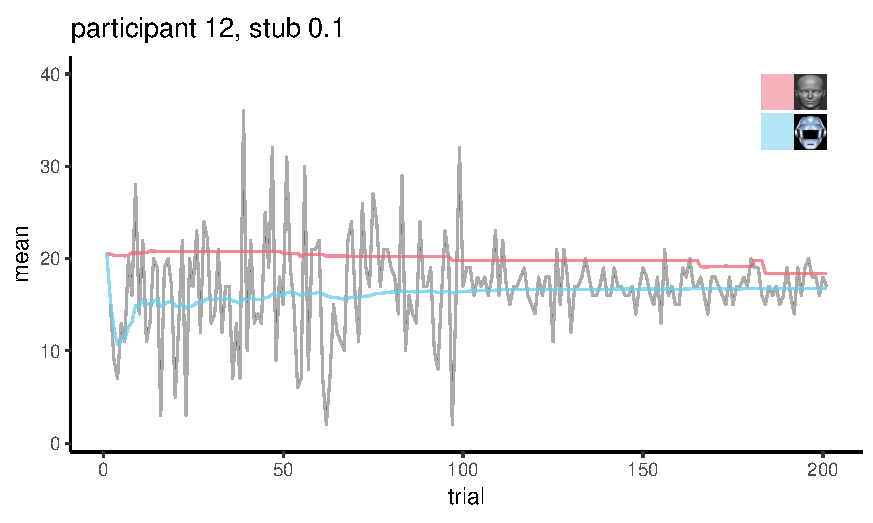
\includegraphics[width=\linewidth]{{comparisons1/means_12-stub_0.1}.pdf}
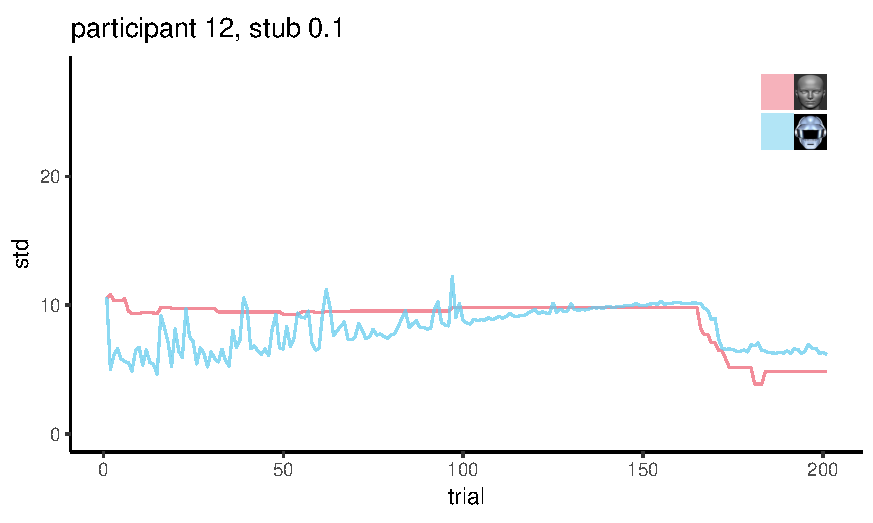
\includegraphics[width=\linewidth]{{comparisons1/stds_12-stub_0.1}.pdf}
\caption{Comparison of the means and standard deviations of the predictive
  distributions of participant~12 and of a robot with stubborness
  $\yN=0.1$}\label{fig:comparison_12_01}
\end{figure}% done with exploration1.R
Figure~\ref{fig:comparison_12_01} shows the means and standard deviations
of the sequence such predictive distributions, for participant~12 and a
robot with stubbornness $\yN=0.1$. This low value makes the robot give
great consideration to the first outcomes, as the initial variability in
the figure shows. The program generating the outcomes had a change in
standard deviation, shifting to a narrower distribution at trial~101. The
robot adapted to this change very slowly.


\begin{figure}[p!]
\centering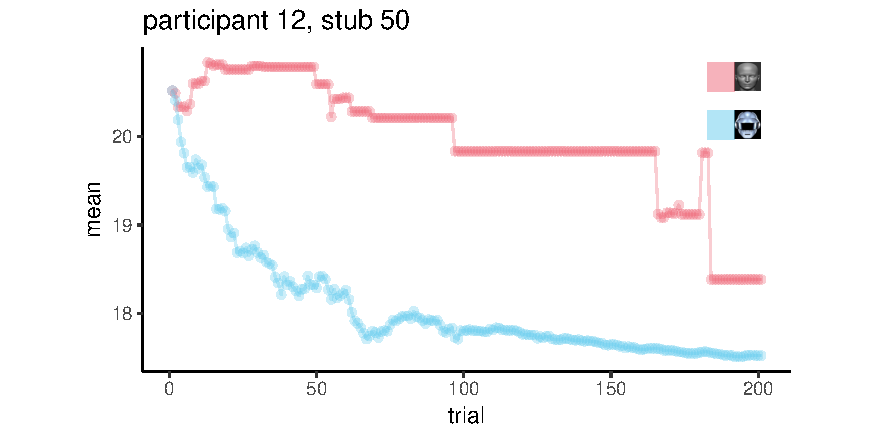
\includegraphics[width=\linewidth]{{comparisons1/means_12-stub_50}.pdf}
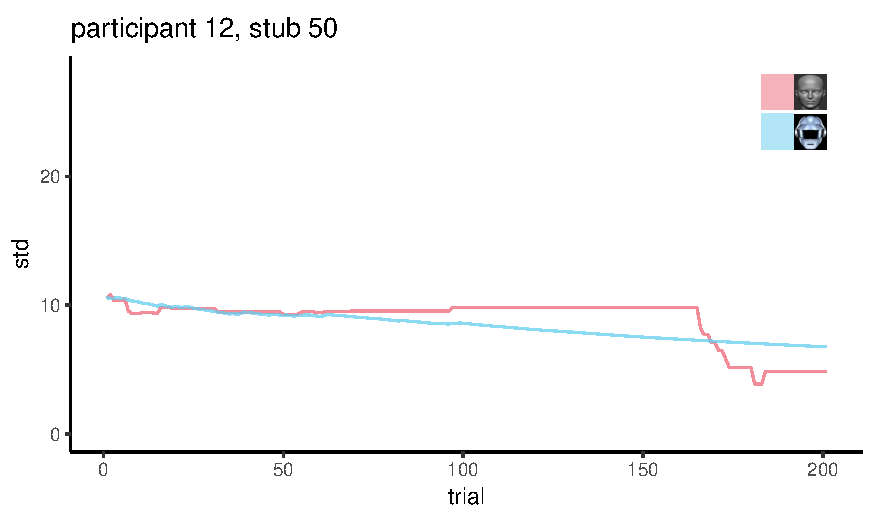
\includegraphics[width=\linewidth]{{comparisons1/stds_12-stub_50}.pdf}
\caption{Comparison of the means and standard deviations of the predictive
  distributions of participant~12 and of a robot with stubborness
  $\yN=50$}\label{fig:comparison_12_50}
\end{figure}% done with exploration1.R
Figure~\ref{fig:comparison_12_50} is analogous to
\fig~\ref{fig:comparison_12_01} but for a robot with stubbornness
$\yN=50$. This robot is even more slow to adapt to the narrowing in the
standard deviation of the generated outcomes.


\begin{figure}[p!]
\centering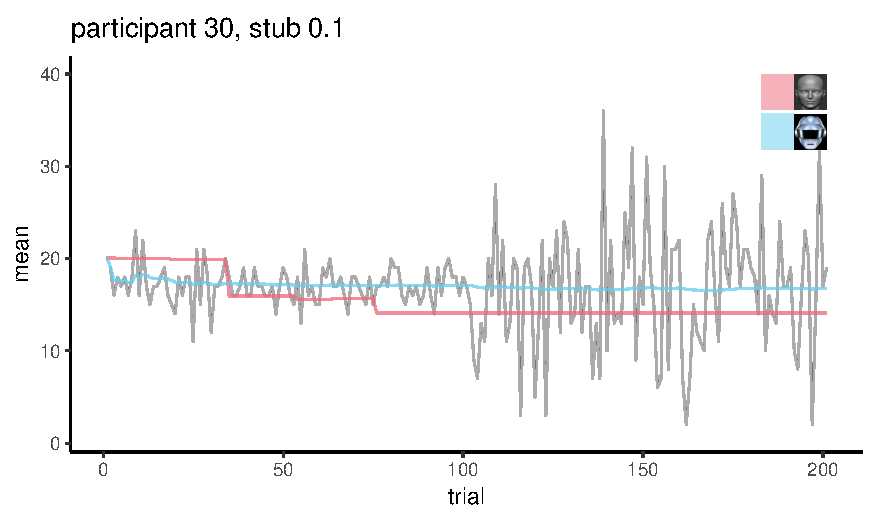
\includegraphics[width=\linewidth]{{comparisons1/means_30-stub_0.1}.pdf}
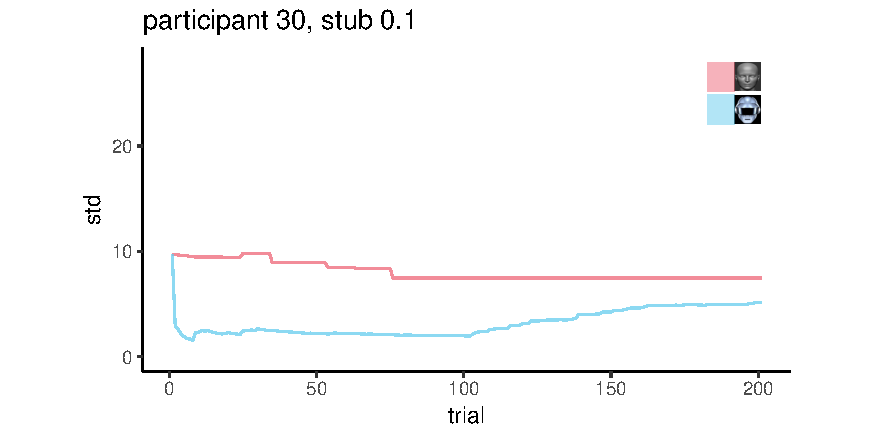
\includegraphics[width=\linewidth]{{comparisons1/stds_30-stub_0.1}.pdf}
\caption{Comparison of the means and standard deviations of the predictive
  distributions of participant~30 and of a robot with stubborness
  $\yN=0.1$}\label{fig:comparison_30_01}
\end{figure}% done with exploration1.R
\begin{figure}[p!]
\centering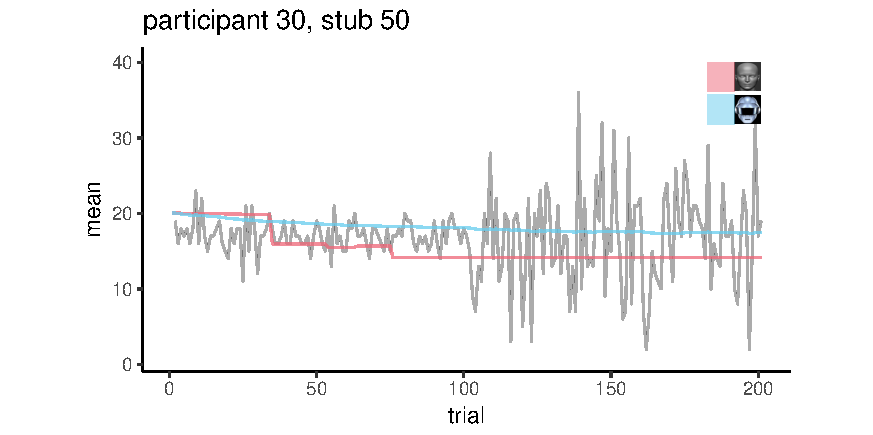
\includegraphics[width=\linewidth]{{comparisons1/means_30-stub_50}.pdf}
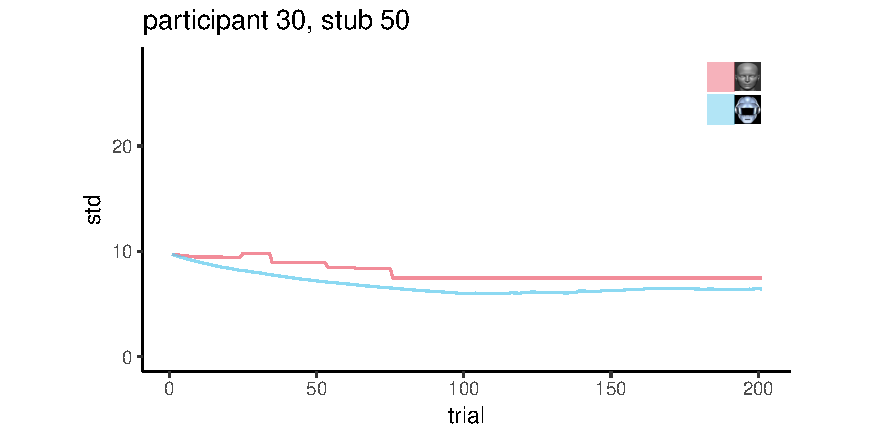
\includegraphics[width=\linewidth]{{comparisons1/stds_30-stub_50}.pdf}
\caption{Comparison of the means and standard deviations of the predictive
  distributions of participant~30 and of a robot with stubborness
  $\yN=50$}\label{fig:comparison_30_50}
\end{figure}% done with exploration1.R
Figures~\ref{fig:comparison_30_01} and~\ref{fig:comparison_30_50} show
the same for participant~30. The change in standard deviation was from
narrow to large in this case.

The robot with low stubbornness seems to adapt to the widening of the
outcome outputs faster than it had for the narrowing of the previous case:
the change in the slope of the robot's standard-deviation curve seems
steeper in \fig~\ref{fig:comparison_30_01} than
in~\ref{fig:comparison_12_01}.


If we look at the sequence of outcomes of \figs~\ref{fig:comparison_12_01}
or~\ref{fig:comparison_30_01}, we perceive that something changed around
trial~100. If we could plot these outcomes while they are generated, we
would likely notice the change by around trial~25. Our robot, however,
can't detect this change for the reasons explained in
\sect~\ref{sec:remarks}; any outcomes from narrow or wide generating
processes are mingled in the robot's memory.

Only non-exchangeable or hierarchic models can exhibit a short evidence
memory and be capable of believing that the underlying \enquote{mechanism}
has changed.


Some conclusions can be drawn from the properties of our model and from the
examples:
\begin{itemize}[para]
\item Participants who have great inertia against updating their
  predictions in view of the observations are \emph{not} necessarily
  behaving at variance with the probability calculus. The latter says that
  they can be as stubborn as they please: larger $\yN$. If we judge such
  inertia as irrational, our judgement cannot be based on such a simple
  model; possibly it's based on a hierarchic model where $\yN$ is given a
  probability that depends on past experiences.

\item The slots have a specific physical order, and from the way the ball
  falls into them it seems reasonable to assume that updates to the
  probability for one slot should affect those for nearby slots. The
  Johnson-Dirichlet model does not take this into account. 

\item A participant who, after observing outcome $k$, raises the bar under
  that slot \emph{and nearby bars} is therefore not acting according to a
  Johnson-Dirichlet exchangeable model.
\item Infinitely exchangeable priors are incapable of quickly adapting to
  changes in the empirical statistics of the outcomes.
\end{itemize}


\section{Examples: robot's surprise}
\label{sec:examples_robot_surprise}

A robot with low stubbornness quickly adapts its predictions to the
observed outcomes, but as the outcomes accumulate its stubbornness
increases. If there is a late change in the generation of the outcomes, at
trial 101 for example, the robot will adapt its predictions more slowly.

It is interesting to ask: is this prediction adaptation the same for a
change from a narrow to a wide distribution, as for a change from a wide to
a narrow one? or is there a difference in the adaptation speed?

The answer depends on how we measure such speed. One way could be this:
starting from the trial in which the change occurs, we let a second robot
with low stubbornness observe the new outcomes and make predictions,
starting from frequency parameters equal to those reached by the first
robot. The second robot will quickly adapt to the new observed outcomes,
and we can use it as a touchstone for the first robot's adaptation speed.
The predictions of the second robot can also be interpreted as if we had
reset the stubbornness of the first robot to a low value.

\begin{figure}[b!]
\centering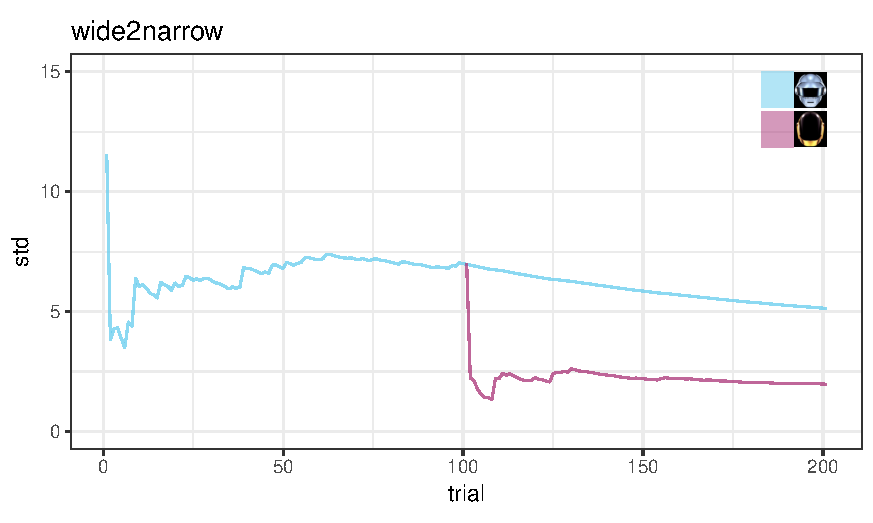
\includegraphics[width=\linewidth]{{comparisons1/compare_robots_wide2narrow-stub_0.1}.pdf}
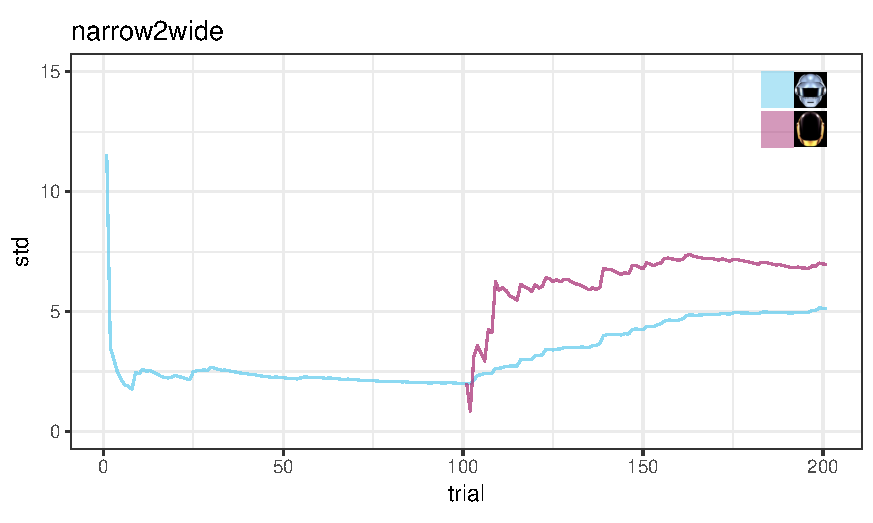
\includegraphics[width=\linewidth]{{comparisons1/compare_robots_narrow2wide-stub_0.1}.pdf}
\caption{Adaptation speed of a robot after a change in the generation of
  the outcomes, compared with that of a robot that starts learning after
  the change. The final relative entropy for the first robot relative to
  the second is $1.01$ in the wide-to-narrow case, vs $0.260$ in the
  narrow-to-wide; exchanging the distributions: $0.283$ vs $0.211$. The
  final overlap is $0.106$ for wide-to-narrow vs $0.0512$ for
  narrow-to-wide}\label{fig:comparison_robots_stds}
\end{figure}% done with exploration1.R
% wide2narrow: relentr=0.2825763, overlap=0.1059542
% narrow2wide: relentr=0.21082114, overlap=0.05119122
The results of this comparison are shown in
\fig~\ref{fig:comparison_robots_stds}. Even though slightly, looking at the
standard deviations of the distributions it seems that a robot adapts more
slowly in going from a wide to a narrow distribution than vice versa. This
is true looking at the final relative entropy of the first robot relative
to the second: $1.01$ wide-to-narrow vs $0.260$ narrow-to-wide; same if we
exchange the distributions: $0.283$ vs $0.211$. The overlap, however, seems
to say the opposite: $0.106$ wide-to-narrow vs $0.0512$ narrow-to-wide.



%\setlength{\intextsep}{0.5ex}% with wrapfigure
%\begin{figure}[p!]%{r}{0.4\linewidth} % with wrapfigure
%  \centering\includegraphics[trim={12ex 0 18ex 0},clip,width=\linewidth]{maxent_saddle.png}\\
%\caption{***}\label{fig:comparison_a5}
%\end{figure}% exp_family_maxent.nb


\iffalse
\begin{acknowledgements}
  \ldots to Mari \amp\ Miri for continuous encouragement and affection, and
  to Buster Keaton and Saitama for filling life with awe and inspiration.
  To the developers and maintainers of \LaTeX, Emacs, AUC\TeX, Open Science
  Framework, Python, Inkscape, Sci-Hub for making a free and unfiltered
  scientific exchange possible.
%\rotatebox{15}{P}\rotatebox{5}{I}\rotatebox{-10}{P}\rotatebox{10}{\reflectbox{P}}\rotatebox{-5}{O}.
%\sourceatright{\autanet}
\end{acknowledgements}
\fi

%\appendixpage
%\appendix

%%%%%%%%%%%%%%% BIB %%%%%%%%%%%%%%%

\defbibnote{prenote}{{\footnotesize (\enquote{de $X$} is listed under D,
    \enquote{van $X$} under V, and so on, regardless of national
    conventions.)\par}}
% \defbibnote{postnote}{\par\medskip\noindent{\footnotesize% Note:
%     \arxivp \mparcp \philscip \biorxivp}}

\printbibliography[prenote=prenote%,postnote=postnote
]


\end{document}
---------- cut text ----------------


%%% Local Variables: 
%%% mode: LaTeX
%%% TeX-PDF-mode: t
%%% TeX-master: t
%%% End: 
